
%Zeitz auskommentiert% \begin{wrapfigure}{l}{0.4\textwidth}         
%\begin{center}           
%                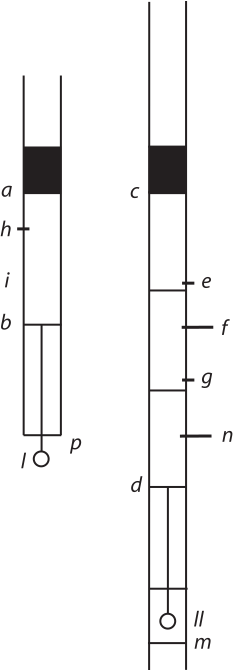
\includegraphics[width=0.26\textwidth]{images/37_3_112r}\\\textit{[Fig. 14]}
%                        %\caption{Bildbeschreibung}
%                        %\end{wrapfigure}
%                        \end{center}
%                        %@ @ @ Dies ist eine Abstandszeile - fuer den Fall, dass mehrere figures hintereinander kommen, ohne dass dazwischen laengerer Text steht. Dies kann zu einer Fahlermeldung fuehren. @ @ @ \\
 \pstart \textso{Theorema:} Si \edtext{duo Elastica (id est tendibilia aut comprimibilia) homogenea}{\lemma{Si}\Afootnote{ \textit{ (1) }\ duo corpora Elastica\protect\index{Sachverzeichnis}{corpus!elasticum|textit} \textit{ (2) }\ duae partes \textit{ (3) }\ duo Elastica  \textit{(a)}\ homogenea \textit{(b)}\ (id [...] homogenea \textit{ L}}} eandem vim perferunt, effectus \edtext{seu spatia in quae comprimuntur}{\lemma{}\Afootnote{seu spatia in quae comprimuntur \textit{ erg.} \textit{ L}}} sunt in duplicata ratione spatiorum, quae vi nulla adhibita ab ipsis implentur. Sunto duo corpora Elastica\protect\index{Sachverzeichnis}{corpus!elasticum} \edtext{homogenea (ut duo aeres) naturaliter implentia hoc}{\lemma{}\Afootnote{homogenea [...] implentia \textit{ (1) }\ aliud spatium \textit{ (2) }\ hoc \textit{ erg.} \textit{ L}}} spatium \textit{ab} illud spatium \textit{cd} quae sunt, ut lineae \textit{ab} $\rule[-4mm]{0mm}{10mm}(\displaystyle\frac{1}{2})$ et \textit{cd} (1) \edtext{cum spatia supponam aequalis}{\lemma{(1)}\Afootnote{ \textit{ (1) }\ aequalis scilicet \textit{ (2) }\ cum spatia supponam aequalis \textit{ L}}} crassitiei ac proinde ut altitudines.\footnote{\selectlanguage{ngerman}\textit{Rechts neben der Zeichnung}: Zwey tubi sollen gleicher weite und die beyden \mercury\ gleich hoch seyn.\selectlanguage{latin}} % \begin{wrapfigure}{l}{0.4\textwidth}                    
                %\includegraphics[width=0.4\textwidth]{../images/Propositio+experimentorum+novorum/LH037%2C03_112r/files/100195.png}
                        %\caption{Bildbeschreibung}
                        %\end{wrapfigure}
                        %@ @ @ Dies ist eine Abstandszeile - fuer den Fall, dass mehrere figures hintereinander kommen, ohne dass dazwischen laengerer Text steht. Dies kann zu einer Fahlermeldung fuehren. @ @ @ \\
                    Pondera duo \textit{a} et \textit{c} comprimentia, aequalia \edtext{(unum quodque 2 librarum)}{\lemma{}\Afootnote{(unum quodque 2 librarum) \textit{ erg.} \textit{ L}}}, et pondus\protect\index{Sachverzeichnis}{pondus} \textit{c} (2 lib.) comprimat corpus \textit{cd} (2) in spatium \textit{de} 
                    $\rule[-4mm]{0mm}{10mm}(\displaystyle\frac{1}{3})$
                     ajo corpus \textit{ab} compressum iri ab eodem pondere in spatium \textit{bi} 
                     $\rule[-4mm]{0mm}{10mm}(\displaystyle\frac{1}{4})$
                      quod sit ad spatium \textit{de} (1) ut est quadratum \textit{ab} (1) ad quadratum \textit{cd} (4). Demonstratio haec est: Sumatur in corpore \textit{cd} pars \edtext{\textit{cf} 
                      $%\rule[-4mm]{0mm}{10mm}
                      (\displaystyle\frac{1}{2})$
                      }{\lemma{}\Afootnote{\textit{cf} $(\protect\frac{1}{2})$ 
                    \textit{ erg.} \textit{ L}}}aequalis corpori $\rule[-4mm]{0mm}{10mm}$\edtext{\textit{ab} $
                    (\displaystyle\frac{1}{2})$,}{\lemma{\textit{ab}}\Afootnote{\textbar\ $(\protect\frac{1}{2})$ 
                    \textit{ erg.} \textbar\ , cujus \textit{ L}}} cujus eadem erit ratio ad \textit{cd} (1) quae est \textit{ab} $\rule[-4mm]{0mm}{10mm}(\displaystyle\frac{1}{2})$ ad \textit{cd} (1) compressione\protect\index{Sachverzeichnis}{compressio} totius \textit{cd} (1) facta in spatium \textit{ed} $\rule[-4mm]{0mm}{10mm}(\displaystyle\frac{2}{3})$ pars \textit{cf} $\rule[-4mm]{0mm}{10mm}(\displaystyle\frac{1}{2})$ compressa est necessario in spatium \textit{eg} $\rule[-4mm]{0mm}{10mm}(\displaystyle\frac{1}{3})$ cujus eadem est ratio ad totum\edtext{}{\lemma{}\Afootnote{totum  \textbar\ novum \textit{ gestr.}\ \textbar\ spatium \textit{ L}}} spatium compressionis\protect\index{Sachverzeichnis}{compressio} \textit{ed} $\rule[-4mm]{0mm}{10mm}(\displaystyle\frac{2}{3})$ quae fuit ante spatii \textit{cf} $\rule[-4mm]{0mm}{10mm}(\displaystyle\frac{1}{2})$ ad totum spatium naturale \textit{cd} (1). Compressa autem est \edtext{haec pars}{\lemma{est}\Afootnote{ \textit{ (1) }\ corpus qu \textit{ (2) }\ haec pars \textit{ L}}} $\rule[-4mm]{0mm}{10mm}(\displaystyle\frac{1}{2})$ quae antea implebat spatium \textit{cf} $\rule[-4mm]{0mm}{10mm}(\displaystyle\frac{1}{2})$  in spatium \textit{eg} $\rule[-4mm]{0mm}{10mm}(\displaystyle\frac{1}{2})$ non tota \edtext{potentia}{\lemma{tota}\Afootnote{ \textit{ (1) }\ vi \textit{ (2) }\ potentia \textit{ L}}} ponderis \textit{c} \edtext{(2 lib.)}{\lemma{}\Afootnote{(2 lib.) \textit{ erg.} \textit{ L}}} sed ejus parte tantum. Quia idem pondus\protect\index{Sachverzeichnis}{pondus} \textit{c} \edtext{(2 lib.)}{\lemma{}\Afootnote{(2 lib.) \textit{ erg.} \textit{ L}}} etiam reliquam totius corporis \textit{cd} (1) partem, nempe \textit{fd} $\rule[-4mm]{0mm}{10mm}(\displaystyle\frac{1}{2})$ in spatium \textit{gd} \rule[-4mm]{0mm}{10mm}\edtext{$(\displaystyle\frac{1}{2})$}{\lemma{}\Afootnote{$(\frac{1}{2})$ \textit{ erg.} \textit{ L}}} compressit. Compressa est ergo pars \textit{cf} in spatium \textit{eg} a parte \edtext{potentiae sibi}{\lemma{parte}\Afootnote{ \textit{ (1) }\ sibi \textit{ (2) }\ potentiae sibi \textit{ L}}} proportionali, seu quae ita sit ad totam potentiam, ut ipsa pars \textit{cf} est ad totam \textit{cd} seu ut spatium \textit{cf} vel \textit{eg} est ad spatium \textit{cd} vel \textit{ed} (seu ut $\rule[-4mm]{0mm}{10mm}\displaystyle\frac{1}{2}$  ad 1) ergo corpus \textit{ab} $\rule[-4mm]{0mm}{10mm}(\displaystyle\frac{1}{2})$ ab eadem vi \edtext{(1 lib.)}{\lemma{}\Afootnote{(1 lib.) \textit{ erg.} \textit{ L}}}, parte scilicet potentiae proportionali in spatium \textit{bh} $\rule[-4mm]{0mm}{10mm}(\displaystyle\frac{1}{2})$ aequale spatio \textit{eg} $\rule[-4mm]{0mm}{10mm}(\displaystyle\frac{1}{3})$ comprimetur. %\edtext{comprimetur.}{\lemma{comprimetur.}\Afootnote{ \textit{ (1) }\ Sed quia vis ipsi  \textit{(a)}\ incumbens est majo \textit{(b)}\ \textit{ab} [...] vi \textit{ L}}}
                    [112 v\textsuperscript{o}] \edtext{Sed quia vis tota ponderis \textit{c} (2 librarum) ipsi \textit{ab} incumbit cum contra non nisi ejus dimidia incubuerit corpori \textit{cf} ideo duplo amplius comprimetur corpus minus \textit{ab}, quam comprimitur pars ei aequalis \textit{cf} in majore}{\lemma{comprimetur.}\Afootnote{ \textit{ (1) }\ Sed quia vis ipsi \textit{(a)} incumbens est majo \textit{(b)} \textit{ab} incumbens est tanto major vi \textit{ (2) }\ Sed [...] comprimetur \textit{(a)}\ quam pars \textit{(b)}\ corpus minus   \textbar\ \textit{ab} \textit{ erg.}\ \textbar\ , quam [...] majore \textit{ L}}} \edtext{seu in spatium dimidium}{\lemma{}\Afootnote{seu in spatium dimidium \textit{ erg.} \textit{ L}}}. Comprimitur autem \textit{cf} in spatium \edtext{\textit{ef}}{\lemma{}\Afootnote{\textit{ef} \textit{ erg.} \textit{ L}}} quod est \edtext{dimidium spatii}{\lemma{est}\Afootnote{ \textit{ (1) }\ tertia pars \textit{ (2) }\ dimidium  \textit{(a)}\ duplo minus quam spatium \textit{(b)}\ spatii \textit{ L}}} \textit{ed} in quod comprimitur solum corpus \textit{ed}. Ideo \edtext{\textit{ab} dimidium corporis \textit{cd} comprimitur}{\lemma{Ideo}\Afootnote{ \textit{ (1) }\ \textit{ab} comprimitur \textit{ (2) }\ \textit{ab} dimidium corporis \textit{cd} comprimitur \textit{ L}}} in dimidium dimidii, seu in quartam partem spatii in quod comprimitur corpus \textit{cd}.\rule[-2cm]{0cm}{1cm} Quod autem in exemplo dicitur in dimidium, id parte ex ratiocinatione esse generaliter in ratione quae est \textit{ab} ad \textit{cd}. Erit ergo pro dimidio dimidii \edtext{substituenda}{\lemma{}\Afootnote{substituenda \textit{ erg.} \textit{ L}}} ratio \textit{ab} ad \textit{cd} duplicata, \edtext{\edlabel{qed112v1}q. e. d.}{\lemma{duplicata,}\Afootnote{ \textit{ (1) }\ seu \textit{ (2) }\ q. e. d. \textit{ L}}}
\edtext{}{\lemma{d.}\xxref{qed112v1}{qed112v2}\Afootnote{ \textit{ (1) }\ Coroll. Hinc si corpus  \textit{(a)}\ unum \textit{(b)}\ aliquod jam sit compressum\protect\index{Sachverzeichnis}{compressio|textit} ad mensurandam novam compressionem\protect\index{Sachverzeichnis}{compressio|textit} seu augmentum comprimentis, auferendum est quantum jam compressum est \textit{ (2) }\ Si [...] sint, \textit{ L}}} 
\pend 